\section{Towards Generic Parallel Programming}\label{chap:background}

A programming model is an abstract representation of a computer. It defines a paradigm and a programming language. The programming language is used by the programmer to write source code, a human readable, textual representation of instructions and data. Source code is a sequential listing of statements evaluated from the top to bottom, one line at a time. While such ordering seems natural to describe an algorithms as it corresponds to sequential processing (both, reading code and progressing the program counter follow a time line), it does not include the notion of concurrency. 

Parallel programming models add the notion of concurrency to a sequence of instruction of a program. This is commonly achieved either by adding semantic value to the base programming language, often referred to as programming with \emph{pragma} annotations, through library calls or new languages. All three approaches are conceptually suitable to represent programming paradigms such as tasking, parallel patterns and others. Well known representatives are the OpenMP programming model~\cite{CITEOPENMP} or threading libraries respectively. In general it is up to the parallel programming model to expose language constructs or library interfaces (APIs) such that they are convenient to the programmer and capture enough semantic information to allow the programming model to map the program execution to the parallel computer hardware efficiently and correctly. Questions of which semantic information is needed, what paradigm to present and by what syntactical means span a design space worth taking a closer look at. Figure~\ref{figSemCapture} shows the three areas that constitute a parallel programming model and its design. We call it the semantic capture.

\begin{figure}[h]
\begin{Verbatim}[frame=leftline]
Semantic information
Paradigm 
Language
\end{Verbatim}
\caption{Semantic capture - a triplet of language, paradigm and semantic information defined by a parallel programming model allow the programmer to express concurrency and the compiler and runtime system to understand and run applications on a parallel machine.}
\label{figSemCapture}
\end{figure}

Semantic information provided by the programmer to the parallel programming model can be grouped into information to express intent and properties. They address the question of \emph{what}, \emph{where} and \emph{how}, which, in the context of parallel programming, corresponds to defining which code portion to parallelize, where to run and access and how to run that parallel code. Synchronization primitives may be considered as part of the what and information on the execution properties such as data placement or memory access type as the how. Semantics are expressed following a paradigm and a programming language.

The parallel programming paradigm is an abstract ~\emph{representation} with the purpose of facilitating the programmer's understanding of programming rules and program behavior. Which programming paradigm to chose depends on several considerations. Parallel-patterns allow to express concurrency for commonly occurring programming patterns such as loop constructs. Tasking is a paradigm that support the expression of concurrent loops as well as irregular algorithms. Distributed and correctness-oriented programming models may implement actor-based programming. In this programming model, each unit of execution represent an actor who communicates over predefined communication interfaces. This paradigm eliminates accesses to shared state and align well with message passing programming (MPI). The execution model and memory model of a programming model defines behavior. That is, it defines the relationship between abstract concepts and program behavior on the given architecture.

Lastly, a language defines the syntax of the parallel semantic. Declarative languages add semantic information to the base language through pragma annotations while imperative languages rely on programming interfaces to capture information. Their semantic is defined in the API specification. Figures~\ref{figOMPLike} and~\ref{figKokkosLike} show examples of two sample applications using the aforementioned parallel programming language types. While both programming models implement the same programming paradigm (parallel patterns), Figures~\ref{figOMPLike} extends the base programming language through pragma annotations. Both, pragma annotations and an API call as shown in Figure~\ref{figKokkosLike} have a similar semantic of describing a parallel loop construct. It is up to the programming model specification to define the execution and memory model in both cases. 

Both examples provide the semantic information on what to parallelize, however, they do not provide information on how to map the parallel execution on modern parallel architectures. In order to define what further information is needed for a generic support on concurrency on modern computer architectures, it is important to define an abstract machine model first.

\begin{figure}
\begin{Verbatim}[frame=leftline]
# pragma model parallel for
for ( size_t i = 0; i < N; ++i) {
 /* loop body */
}
\end{Verbatim}
\caption{Declarative parallel programming provides uses pragma annotations to capture semantic information.}
\label{figOMPLike}
\end{figure}

\begin{figure}
\begin{Verbatim}[frame=leftline]
model::parallel_for (N, [=] ( const size_t i) {
  /* loop body */
});
\end{Verbatim}
\caption{Imperative parallel programming uses a base language and relies on programming interfaces to capture information and a documentation that describe their semantics.}
\label{figKokkosLike}
\end{figure}

\section{The Kokkos Abstract Machine Model}\label{chap:kokkosMM}

The Kokkos machine model defines abstractions that represent hardware capabilities for processing and data access. The Kokkos parallel programming model exposes these abstractions to the programmer through C++ and the Kokkos API. By abstracting from physical hardware, the machine model ensures that applications written in programming models targeting this machine model are generic and performance-portable on current and future hardware. The Kokkos parallel programming model is one particular instance of a programming model that builds on top of that machine model. We would like to point out that it is this conceptual differentiation that allows scenarios where the underlying machine model is instantiated in other languages beyond C++, yet the algorithmic specification as well as performance characteristic and portability remain the same. 

The Kokkos abstract machine model targets a design of a future shared-memory computing architectures. The design is shown in Figure~\ref{fig:execspace}. It is characterized by multiple latency-optimized execution units and off-die bandwidth-optimized accelerators. Both compute device types have disjoint memory address spaces and unique performance properties. In such an architecture,   execution units might be grouped into larger units with multiple levels of achievable parallelism with different memory access characteristics and coherence properties of caches. In order to ensure performance portability on such a wide range of configurations, an abstraction of the compute engines and available memories are required. For this purpose we introduce \emph{spaces}.

An instance of an \emph{execution space} is a specific instantiation of an execution space to which a programmer can target parallel work. For example, an execution space can be used to describe a multi-core processor. In this case, the execution space contains several homogeneous cores organized into arbitrary logical groups. In a parallel programming model that implements this machine model, an instance of such an execution space would be made available to the programmer to run kernels. Adding more logical groups or accelerators simply increases the number of available execution spaces to the programmer.

Memory and memory types are exposed through \emph{memory spaces}. Each memory space provides a finite storage capacity at which data structures can be allocated and accessed. Different memory space types have different characteristics with respect to accessibility from execution spaces and performance. 

An instance of a memory space provides a concrete method for the application programmer to request data storage allocations. Following the architecture as discussed earlier, the multi-core processor may contain multiple memory spaces that abstract on-package memory, slower DRAM and non-volatile memories. Accelerators can provide an additional memory space through its local on-package memory. The programmer is free to decide where each data structure is allocated by requesting the corresponding memory space by instantiating the according memory space. Kokkos provides the appropriate abstraction of memory allocation and data management. We believe that an abstract representation of execution- and memory devices is a key property towards performance-portable parallel programming.

How a machine model is exposed to the programmer and what are the design considerations towards defining an appropriate semantic capture are discussed in the next section.

%Ang, J.A., et. al., Abstract Machine Models and Proxy Architectures for Exascale Computing, 2014, Sandia National Laboratories and Lawrence Berkeley National Laboratory, DOE Computer Architecture Laboratories Project


\begin{figure}
\begin{subfigure}[b]{0.45\textwidth}
\centering
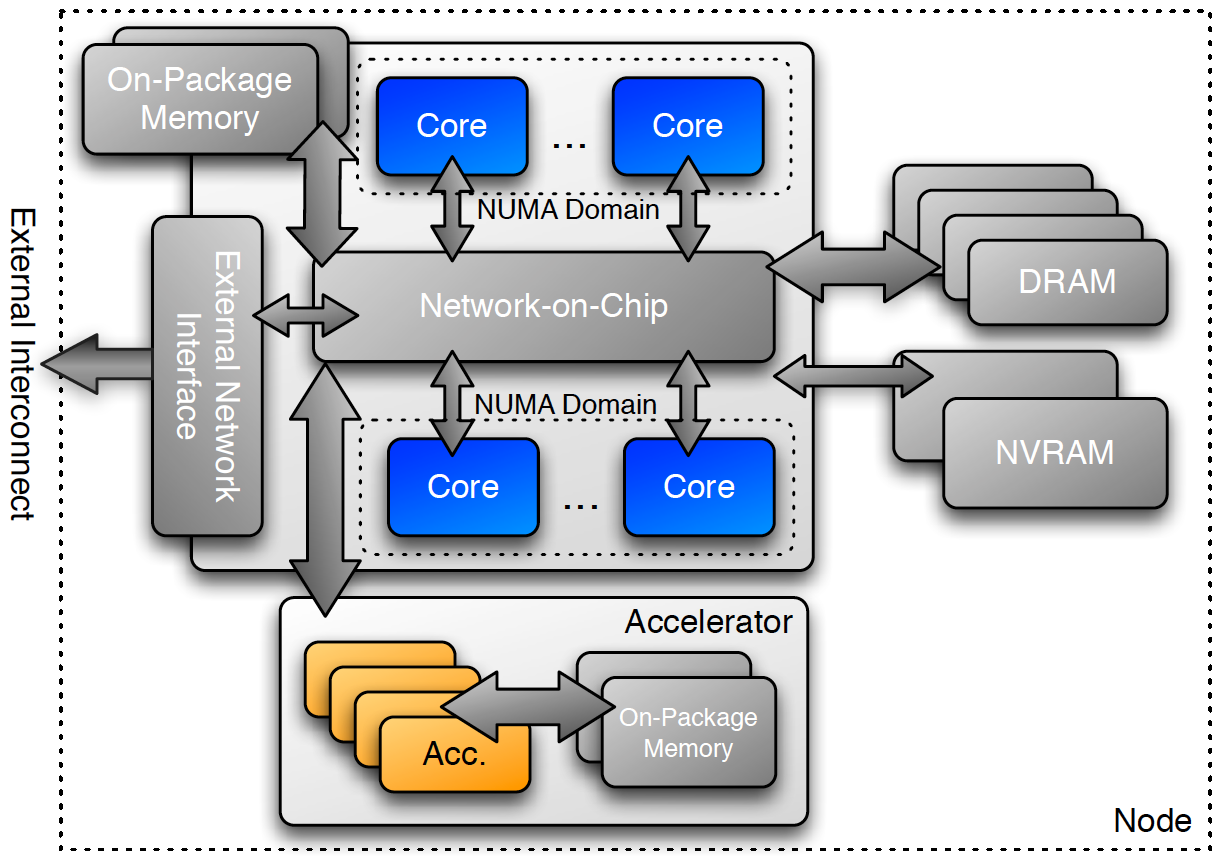
\includegraphics[width=\textwidth]{img/ExecSpaces.png}
\caption{Execution space is an instantiation of a space that represents a processing device to which the programmer can target parallel code.}
\label{fig:execspace}
\end{subfigure}%
\hfill \break
\begin{subfigure}[b]{0.45\textwidth}

\centering
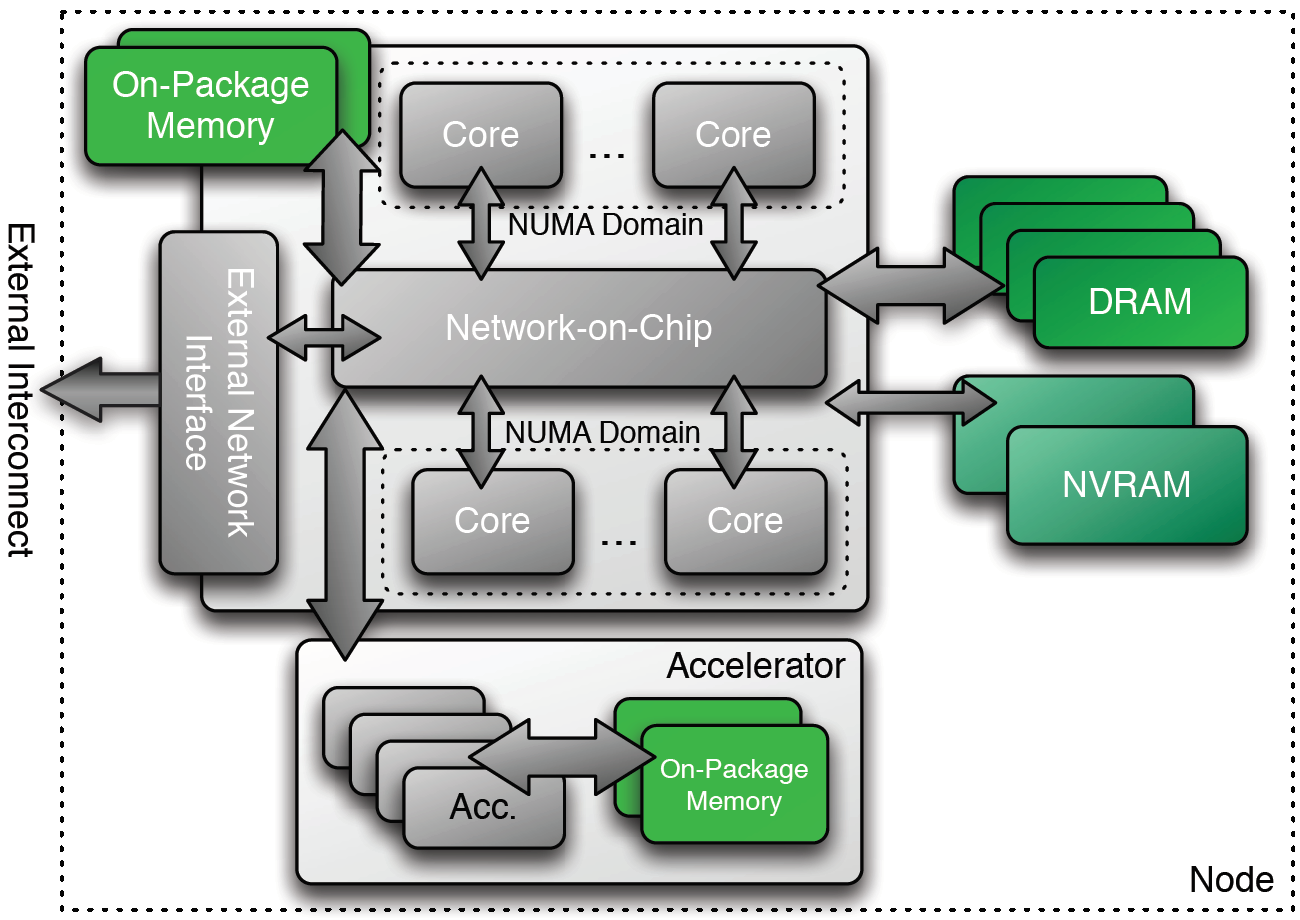
\includegraphics[width=\textwidth]{img/MemSpaces.png}
\caption{A memory space is an instantiation of a space that represents a memory location on which the programmer can allocate data.}
\label{fig:memspace}
\end{subfigure}%
\caption{Spaces represent conceptual building blocks of the abstract machine model in Kokkos.}
\label{fig:spaces}
\end{figure}

\section{The Kokkos Programming Model}\label{chap:kokkosPM}
%====================

%The Kokkos programming model defines a programming language, paradigm and semantic information. Its design has been motivated by the desire to develop a generic, performance portable programming model that would be convenient enough to the programmer and allow a runtime library to map programming concepts and execution to the underlying abstract machine model at the same time. We take a closer look as follows.
The Kokkos programming model specifies a language, programming paradigm and an API that captures intents and properties of execution. This completes the semantic capture, discussed in Chapter~\ref{chap:background}, which allows the expression of concurrency and efficient program execution on the underlying hardware. We detail all three comments as follows.

Kokkos defines a pure interface for C++ and uses C++ as the base programming language. This has multiple reasons. Firstly, application developers of scientific and high-performance computing applications at Sandia National Laboratories expressed the demand for C++ and a generic programming model in order to support their codes. Following their estimates, code porting to changing vendor APIs represents an anacceptable burden and the possibility to  

Other reasons exist. From the implementation persoecte, C++ allows meta programming which is well suited to implement generic APIs and libraries. In this case, class specialization and teplating allows to compiler-generate optimized intefaces libraries for a given underlying hardware architecture. This effectively allows for compile time transformation of algorithms to allow for adaptions of varying degrees of hardware parallelism as well as of the memory hierarchy.
Consequently, while Kokkos targets C++, we believe that any programming language can be used to express the paradigms and semantic information to efficenly support the abstravt machine model.

Kokkos supports the parallel patterns and task paradigms. Parallel patters covers \emph{for}, \emph{ scan} and \emph{reduction}. This allows the expression on concurrency over iterative, for-loop computable algorithms. To cover the class of while-loop computable algorithms (irregular algorithms), Kokkos implements the tasking paradigm. Tasks encapsulate work into units that may be executed in parallel to other tasks or sections of the program.

These  concepts allow the formulation of generic algorithms and data structures which can then be mapped to different types of architectures. Effectively, they allow for compile time transformation of algorithms to allow for adaptions of varying degrees of hardware parallelism as well as of the memory hierarchy.


C++ because popular (perf critical code in industry)
Use-case (SNL)
Language features are present and first-class citizen. 
Allow to make the PM as part of the language -> type information | overloading ops
No Source2source compiler needed
Template mechanisms / type / meta info: to write abstractions 
template meta programming privde a library to implement the progamming mdoel
- pure way to suppport the machine model
- not tide to a specific implementation of underlying hardware
- No additional semantics through pragma annotations

\section{Kokkos Abstractions}

To capture semantic information, that is the~\emph{What}, the ~\emph{Where} and the ~\emph{How}, Kokkos introduces  six abstractions: \emph{execution spaces}, \emph{execution patterns}, \emph{execution policies}, \emph{memory spaces}, \emph{memory layout} and \emph{memory traits}. These abstractions specify semantic information and enable the runtime to efficiently map the program to any underlying hardware architecture represented by abstract machine model. We take a closer look as follows.

An execution space is a place where code can be executed. On current hardware architectures this correspond to accelerators and CPUs. In the future this can include Processing in Memory (PIM) modules or different core types on a heterogeneous CPU. This model allows to include computing elements In principle, execution spaces can include remote execution spaces to support e.g., the capability of sending work to a different node. Execution Spaces thus give an application developer the means to target different parts of a heterogeneous hardware architecture. This corresponds directly to the previously described machine model.

Execution patterns are the fundamental parallel algorithms in which an application has to be expressed. Examples are the parallel\_for: execute a function in undetermined order a specified amount of times,
parallel\_reduce: which combines a parallel\_for execution with a reduction operation,
parallel\_scan: which combines a parallel\_for operation with a prefix or postfix scan on output values of each operation, and
task: which executes a single function with dependencies on other functions.
Expressing an application in these patterns allows the underlying implementation or the used compiler to reason about valid transformations. For example all parallel\_*** patterns allow unspecified execution order and only promise deterministic results of the reductions themselves. This enables different mapping patterns on different hardware such as assignment of iterations to threads or vector lanes.

An execution policy determines, together with an execution pattern, how a function is executed. Some policies can be nested in others. The most simple form of execution policies are range policies. They are used to execute an operation once for each element in a range. There are no prescriptions of order of execution or concurrency, which means that it is not legal to synchronize different iterations.

Team policies are used to implement hierarchical parallelism. For that purpose Kokkos groups threads into teams. A thread team is a collection of one or more parallel "threads" of execution. Kokkos allows an arbitrary number of teams - the league size. Hardware constrains the number of threads in a team - the team size. All threads in a team are guaranteed to run concurrently.

Memory spaces are the places where data resides. They specify physical location of data as well as access characteristics. Different physical locations correspond to different device types such as high bandwidth memories, on-die scratch memories or non-volatile bulk storage. Different logical memory spaces allow for concepts such as UVM memory in the CUDA programming model, which is accessible from the host and the CUDA accelerator. Memory Spaces, similarly to execution spaces, conceptually support remote memory locations in distributed-memory scenarios. Furthermore, they encapsulate functionality such as consistency control and persistence scopes.

Layouts express the mapping from logical (algorithmic) indices to address offset for a data allocation. By adopting appropriate layouts for memory structures, an application can optimize data access patterns in a given algorithm. If an implementation provides polymorphic layouts (i.e. a data structure can be instantiated at compile or runtime with different layouts), an architecture dependent optimization can be performed.

Memory traits specify how a data structure is accessed in an algorithm. Traits express usage scenarios such as atomic access, random access and streaming loads or stores. By putting such attributes on data structures, an implementation of the programming model can insert optimal load and store operations. If a compiler implements the programming model, it could reason about the access modes and use that to inform code transformations.

These concepts allow the generic formulation of algorithms and data structures that can be mapped to the any hardware architecture that can be abstracted through the machine model.. Effectively, they allow for compile time transformation of algorithms to allow for adaption of varying degrees of hardware parallelism as well as of the memory hierarchy.


%\begin{figure}
%\begin{Verbatim}[frame=leftline]
%T main(int argc, char** argv)
%{
% agent<T> a, b;
% a.SetInput(b.GetOutput());
% a.start();
% b.start();
% agent::wait(&a);
% return a.out();
%}
%\end{Verbatim}
%\caption{The actor-based programming paradigm builds upon the idea of isolation and message-passing which is considered a contribution towards helping developers to write correct code, to express unstructured parallelism and to support the execution on distributed memory systems.}
%\label{figAgentsLike}
%\end{figure}

\begin{figure}[h]
\begin{Verbatim}[frame=leftline]
Semantic information: Patterns (intent), Spaces, Layouts, 
Policies and Traits
Paradigm: Parallel patterns and tasking
Language: C++
\end{Verbatim}
\caption{Semantic capture defining the Kokkos programming model.}
\label{figSemCapture}
\end{figure}

\begin{figure}
\begin{Verbatim}[frame=leftline]
parallel_for <ExecutionSpace<>>
parallel_scan <>
parallel_reduce <>
task <>
\end{Verbatim}
\caption{The Kokkos programming model uses template meta programming to specialize types for  exposes concurrency through parallel patterns and tasking in the C++ base language.}
\label{fig}
\end{figure}

%\begin{center}
%\begin{tabular}{ |c|c|c| } 
% \hline
% cell1 & cell2 & cell3 \\ 
% cell4 & cell5 & cell6 \\ 
% cell7 & cell8 & cell9 \\ 
% \hline
%\end{tabular}
%\end{center}

%\begin{figure}
%\begin{Verbatim}[frame=leftline]
%double f(){
% typedef Kokkos::Cuda ES;
% typedef Kokkos::CudaSpace MS;
% typedef Kokkos::LayoutLeft LL;
% typedef Kokkos::RangePolicy<ES> Range_policy;
% typedef Kokkos::View<double*, LL, MS> V
% V A( "A", N);
% V::HostMirror h_A = Kokkos::create_mirror_view( A );
% for ( int i = 0; i < N; ++i ) //Initialize on host
%   h_A( i ) = 1;
% Kokkos::deep_copy( A, h_A );
% double result = 0;
% Kokkos::parallel_reduce( "yAx", range_policy( 0, N ), 
%  KOKKOS_LAMBDA ( int i, double &update ) {
%   update += A( i );
% }, result );
% return result;
%}
%\end{Verbatim}
%\caption{Declarative parallel programming provides uses pragma annotations to capture semantic information.}
%\label{figOMPLike}
%\end{figure}

%machine model 

%\begin{figure}
%\centerline{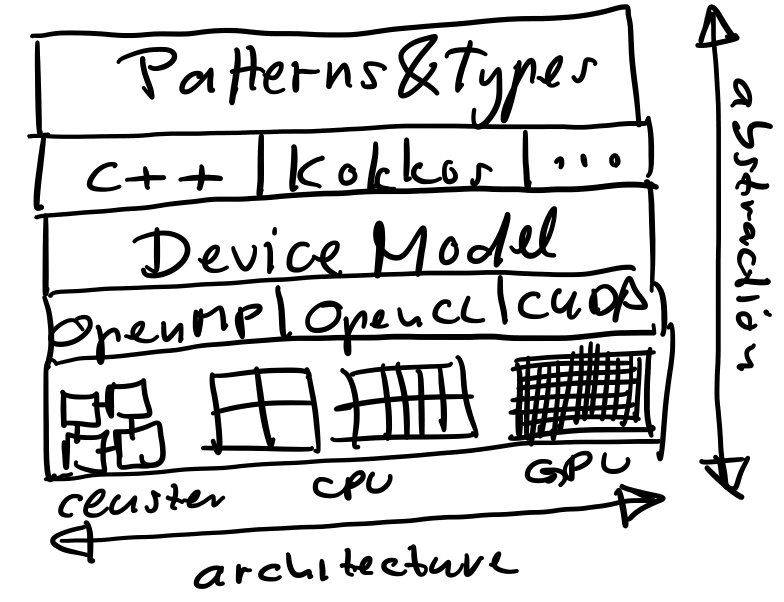
\includegraphics[width=0.4\textwidth]{img/Stack.png}}
%\caption{Stack}
%\label{fig}
%\end{figure}

%\begin{figure}
%\centerline{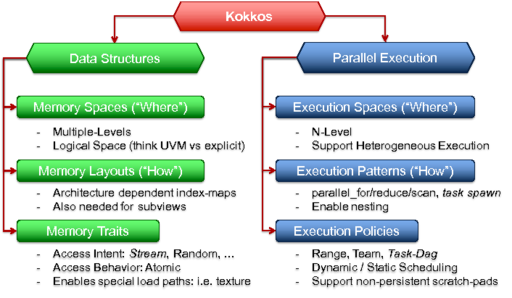
\includegraphics[width=0.4\textwidth]{img/Abstractions.png}}
%\caption{Building workflow}
%\label{fig}
%\end{figure}

\begin{figure}
\centerline{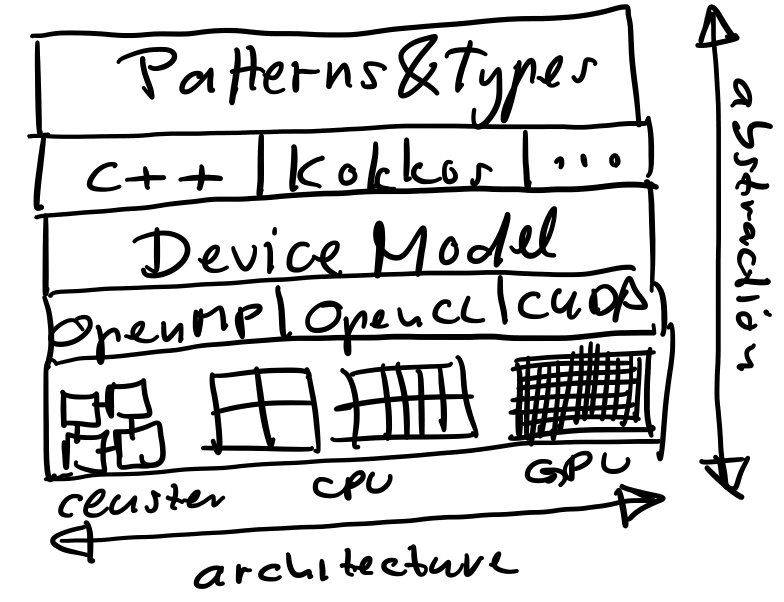
\includegraphics[width=0.4\textwidth]{img/Stack.png}}
\caption{Landscaoe}
\label{fig:stack}
\end{figure}


The Kokkos semantic capture des


 While design choices regarding the language and programming paradigm address requirements posed by developers in scientific computing, the set semantic information required is defined by the need to support the abstract machine model. 

Figure\ref{fig:stack} shows abstraction layers in Kokkos and its fit in a parallel programming landscape.
The next Chapter shows an example application written in Kokkos and provides an insight into the runtime library.


\section{Back-end Support}\label{chap:kokkosBackend}


The important consideration here is that the method of compiling code for different execution spaces and the dispatch of kernels to instances is abstracted by the Kokkos model. This unburdens application programmers from writing algorithms in hardware specific languages.


\begin{figure}
\centerline{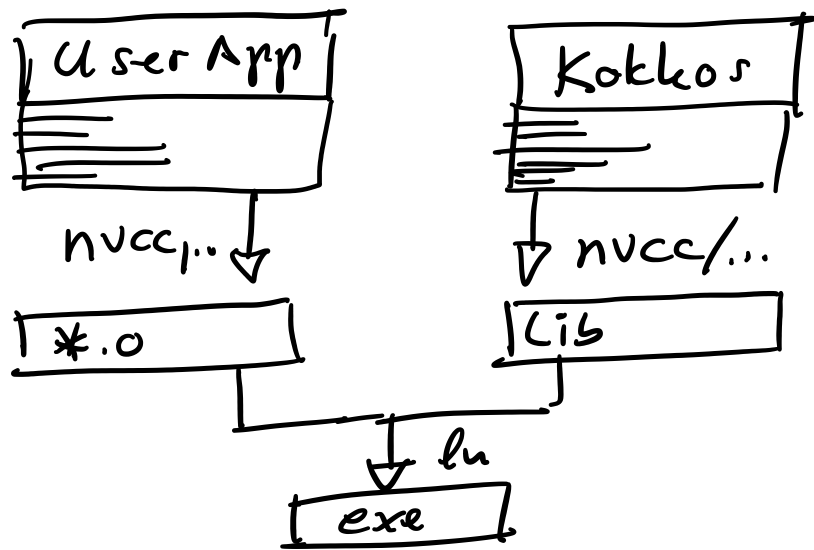
\includegraphics[width=0.4\textwidth]{img/Build.png}}
\caption{Building workflow}
\label{fig}
\end{figure}

